\section{Influence on Detection Rate}
\label{sec:corr}
In this section, we study factors influencing detection rate of PE submissions. 
Our study is conducted from 4 aspects: reputation of source id, submission history, 
file size, and source country.

\subsection{Reputation of Source ID}



\begin{figure}[t!]
\begin{center}
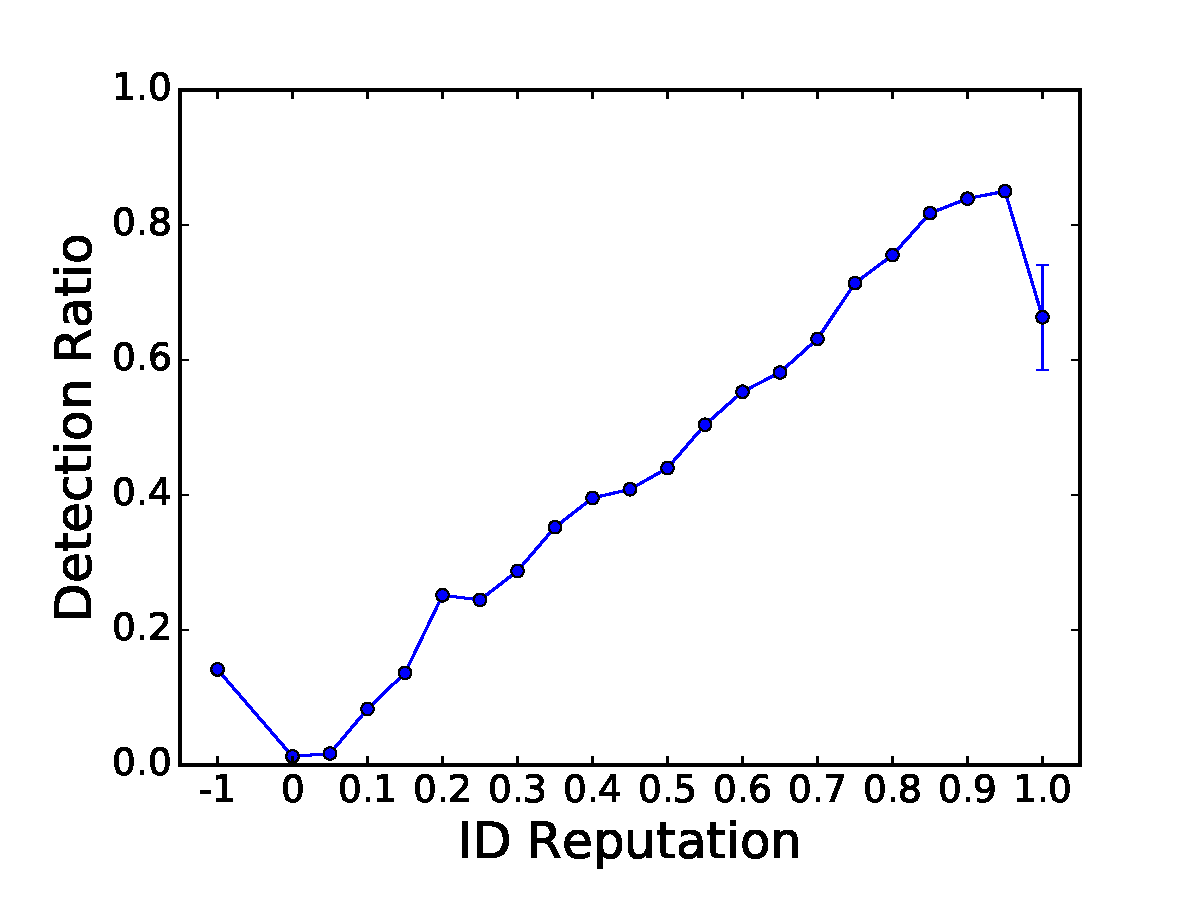
\includegraphics[width=2.5in]{figure/IDReputation}
\mycaption{fig:idreputation}{The relation between source id's previous reputation and detection rate.}
{\footnotesize{(How detection rate changes with the value of source id's reputation. Each reputation is rounded up to nearest 0.05.
Reputation -1 means the source id did not make any submission before. 95\% confidence interval is also drawn 
for each point.)}}
\end{center}
%\vspace{-0.25in}
\end{figure}


Previous work~\cite{GuoICSE2010} reported correlation between bug reporter’s reputation and the likelihood for the bug being fixed. 
We also observe correlation between the reputation of source id and submission’s detection rate. 

%\theoremstyle{definition}
\begin{definition}{Reputation:}
Given a submission $S$ with source id $I$, 
we define the reputation of $I$ when conducting the submission $S$ as the average detection rate for all submissions conducted by $I$ before $S$. 
If $I$ did not make any submission before, we define the reputation to be $-1$. 
\end{definition}

For around 14\% PE submissions, VirusTotal fails to provide source id information. 
We filter out these submissions, when computing reputation.
All other PE submissions are conducted by 613 thousand source ids. 
More than half source ids (66\%) only conduct submission once. 
We filter source ids conducting more than 1 million PE submissions in our data set, 
because we think these are anti-virus vendors routinely test their products. 

When calculating reputation, we sort all submissions from the same source id chronologically, 
and calculate reputation for the id when conducting each submission. 
We round up each calculated reputation to nearest 0.05. 
We group submissions based on source ids' reputation when conducting submissions, 
and we plot average detection rate and 95\% confidence interval for each group in Figure~\ref{fig:idreputation}. 
Except the point with reputation 1, all other confidence intervals are invisible.  

As shown in Figure~\ref{fig:idreputation}, 
there is a rough increase for detection rate as the increase of source id's reputation, 
with the exception for the point with reputation -1 and the point with reputation 1. 
It is interesting to observe that first submissions conducted by different source ids have higher 
detection rate than submissions conducted by ids with reputation 0, 
and it is difficult for source ids with highest reputation to keep highest reputation.  

{\bf TODO: ADDING A SMALL DISCUSSION PARAGRAPH}

\subsection{Submission History}